\documentclass{article}
\usepackage[utf8]{inputenc}
\usepackage{geometry}
\geometry{a4paper, margin=1in}
\usepackage{hyperref}
\usepackage{enumitem}
\usepackage{tikz}
\usetikzlibrary{shapes.geometric, arrows, positioning}
\tikzstyle{startstop} = [rectangle, rounded corners, minimum width=3cm, minimum height=1cm,text centered, draw=black, fill=red!30]
\tikzstyle{process} = [rectangle, minimum width=3cm, minimum height=1cm, text centered, draw=black, fill=orange!30]
\tikzstyle{decision} = [diamond, minimum width=3cm, minimum height=1cm, text centered, draw=black, fill=green!30]
\tikzstyle{arrow} = [thick,->,>=stealth]

\title{Suspicious Activity Report Generator with Audit Trail}
\author{}
\date{}

\begin{document}

\maketitle

\section{Abstract}
Financial institutions are mandated to file Suspicious Activity Reports (SARs) for potential financial crimes, a process that is currently manual, labor-intensive (taking 5–6 hours per report), and prone to inconsistency. This project proposes a Suspicious Activity Report Generator with an integrated Audit Trail and Active Learning loop. By leveraging Large Language Models (LLMs) and Retrieval-Augmented Generation (RAG), the system automates the drafting of regulator-ready narratives using transaction alerts and customer KYC data. Crucially, it addresses the "black box" problem of AI by providing a transparent audit trail and employs a feedback mechanism where analyst corrections retrain the underlying risk models, creating a self-improving system. This solution aims to drastically reduce compliance backlogs, ensure standardized reporting, and free up analysts to focus on complex investigations.

\section{System Architecture}
The system is architected as a set of loosely coupled microservices, ensuring modularity and flexibility.
\begin{enumerate}
    \item \textbf{API Gateway (Ingress)}: Serves as the single entry point, handling authentication (OAuth2/OIDC), rate limiting, and request routing to appropriate backend services.
    \item \textbf{Data Ingestion Service}: aggregated structured data (transaction alerts from core banking) and unstructured data (KYC documents, emails). It utilizes Apache Kafka for high-throughput, fault-tolerant data streaming.
    \item \textbf{Context \& Knowledge Engine (RAG)}:
    \begin{itemize}
        \item \textbf{Vector Database}: ChromaDB running in a Docker container. Stores embedding vectors of regulatory guidelines (FinCEN/FCA) and historical SARs.
        \item \textbf{Retrieval Service}: Semantically searches the vector store to fetch relevant context for the current case.
    \end{itemize}
    \item \textbf{Generative Core Service}:
    \begin{itemize}
        \item Hosts the LLM (Llama 3.1 8B/70B) utilizing vLLM or TGI for optimized inference.
        \item Processes the prompt constructed from the alert data and retrieved context.
    \end{itemize}
    \item \textbf{Explainability \& Audit Service}: Intercepts the generation process to map output tokens back to source documents, creating a citation chain saved to an immutable audit log.
    \item \textbf{Frontend Application}: A React/Streamlit-based dashboard for analysts to view alerts, generate drafts, review the audit trail, and submit final reports.
    \item \textbf{Active Learning & Feedback Engine}: Captures analyst modifications to generated narratives and labeled case outcomes (True/False Positive). This structured feedback is used to incrementally retrain the XGBoost risk model and fine-tune the LLM, ensuring the system adapts to evolving financial crime typologies.
\end{enumerate}

\section{Fraud Detection \& Active Learning Pipeline}
This section details the specialized machine learning workflow designed to filter transactions with high precision before they reach the generative AI layer.

\begin{figure}[h]
\centering
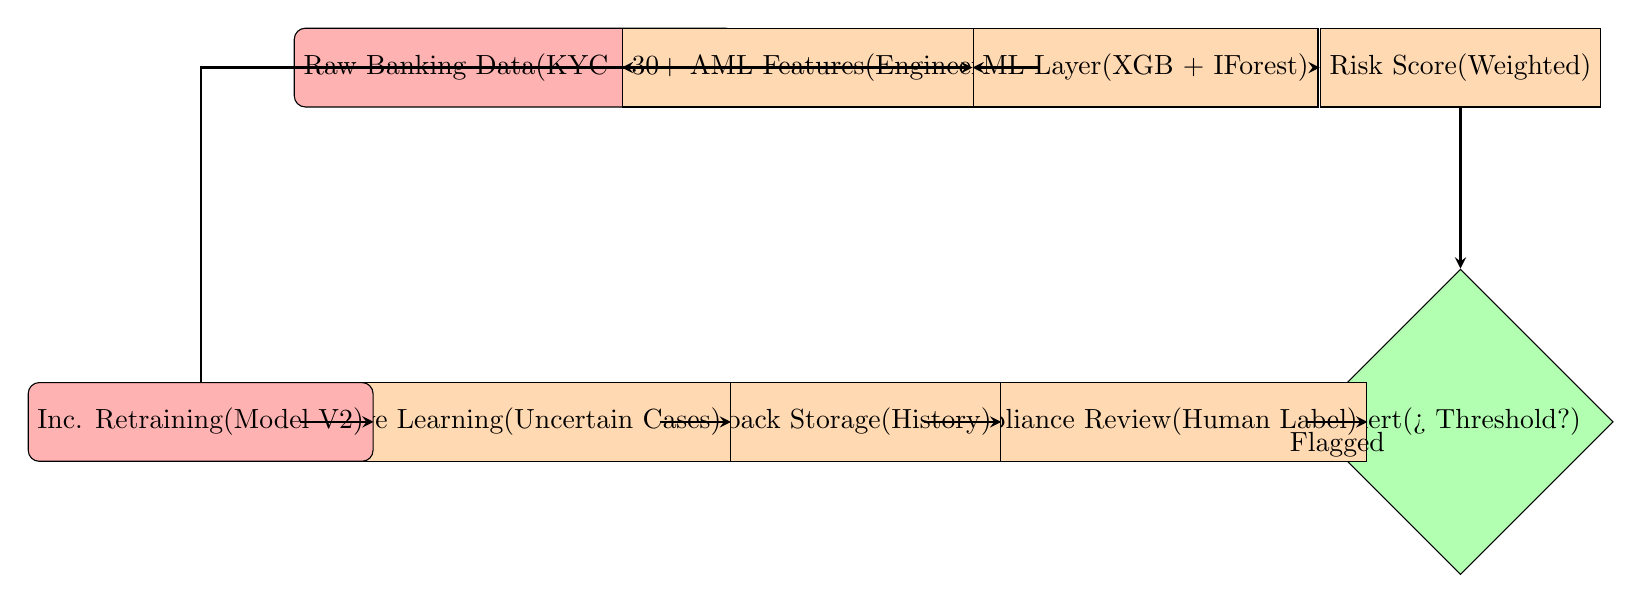
\begin{tikzpicture}[node distance=3cm]
% Row 1
\node (raw) [startstop] {Raw Banking Data\\(KYC + Trans)};
\node (feat) [process, right of=raw, xshift=1cm] {30+ AML Features\\(Engineering)};
\node (ml) [process, right of=feat, xshift=1cm] {ML Layer\\(XGB + IForest)};
\node (score) [process, right of=ml, xshift=1cm] {Risk Score\\(Weighted)};

% Row 2
\node (alert) [decision, below of=score, yshift=-1.5cm] {Alert\\(> Threshold?)};
\node (review) [process, left of=alert, xshift=-1cm] {Compliance Review\\(Human Label)};
\node (feedback) [process, left of=review, xshift=-1cm] {Feedback Storage\\(History)};
\node (active) [process, left of=feedback, xshift=-1cm] {Active Learning\\(Uncertain Cases)};
\node (retrain) [startstop, left of=active, xshift=-1cm] {Inc. Retraining\\(Model V2)};

% Draw Arrows
\draw [arrow] (raw) -- (feat);
\draw [arrow] (feat) -- (ml);
\draw [arrow] (ml) -- (score);
\draw [arrow] (score) -- (alert);
\draw [arrow] (alert) -- node[anchor=north] {Flagged} (review);
\draw [arrow] (review) -- (feedback);
\draw [arrow] (feedback) -- (active);
\draw [arrow] (active) -- (retrain);

% Loop back
\draw [arrow] (retrain) |- (ml);

\end{tikzpicture}
\caption{End-to-End Fraud Detection Workflow with Active Learning Loop}
\label{fig:fraud_pipeline}
\end{figure}

The pipeline consists of the following key stages:
\begin{itemize}
    \item \textbf{Feature Engineering}: Transforms raw data into behavioral indicators (e.g., velocity, deviation from profile).
    \item \textbf{ML Layer}: Utilizes a hybrid approach with \textbf{XGBoost} (Supervised Learning) for known patterns and \textbf{Isolation Forest} for detecting novel anomalies.
    \item \textbf{Risk Aggregation}: Combines scores from multiple models into a single weighted risk score.
    \item \textbf{Active Learning}: Automatically identifies "uncertain" cases (those near the decision boundary) for human review, using the feedback to incrementally retrain and improve the model over time.
\end{itemize}
\section{Methodology: Scalability, Performance, and Security}
\subsection{Scalability}
The system is designed for massive scale to handle surges in transaction alerts.
\begin{itemize}
    \item \textbf{Horizontal Pod Autoscaling (HPA)}: All microservices are containerized (Docker) and orchestrated via Kubernetes. HPA automatically scales the number of replica pods based on CPU/Memory usage or custom metrics (e.g., Kafka lag).
    \item \textbf{Database Sharding}: The PostgreSQL database used for case management employs sharding (e.g., via Citus) to distribute data across multiple nodes, ensuring high read/write throughput.
    \item \textbf{Asynchronous Processing}: Long-running generation tasks are handled asynchronously using task queues (Celery/Redis), preventing API blocking.
\end{itemize}

\subsection{Performance}
\begin{itemize}
    \item \textbf{Quantization}: We use 4-bit or 8-bit quantized models (AWQ/GPTQ) to reduce memory footprint and increase inference speed without significant accuracy loss.
    \item \textbf{Caching}: Redis is used to cache frequent vector search results and repetitive queries, reducing load on the vector DB and LLM.
    \item \textbf{gRPC}: Inter-service communication uses gRPC (Protobuf), which is lighter and faster than REST/JSON.
\end{itemize}

\subsection{Security}
\begin{itemize}
    \item \textbf{Data Sovereignty}: Complete on-premise or private cloud deployment ensures no data leaves the institution's secure perimeter.
    \item \textbf{Encryption}: TLS 1.3 for data in transit; AES-256 for data at rest (database and vector store volumes).
    \item \textbf{RBAC}: Granular Role-Based Access Control limits access. Only authorized compliance officers can view PII or generic reports.
\end{itemize}

\section{Tech Stack}
\begin{itemize}
    \item \textbf{LLM}: Llama 3.1 (8B) or Mistral 7B via Ollama/vLLM
    \item \textbf{Orchestration}: LangChain / LlamaIndex
    \item \textbf{Vector Database}: ChromaDB (Containerized on Docker)
    \item \textbf{Backend}: Python (FastAPI/Django), gRPC
    \item \textbf{Frontend}: Streamlit / React JS
    \item \textbf{Database}: PostgreSQL (Case Management), Redis (Caching)
    \item \textbf{Infrastructure}: Docker, Kubernetes, Helm
\end{itemize}

\section{Deployment Strategy: On-Premise vs. Cloud}
The solution supports a hybrid deployment model, allowing institutions to transition from on-premise to cloud at their own pace.

\subsection{On-Premise Deployment}
\begin{itemize}
    \item \textbf{Infrastructure}: Deployed on bare-metal servers or local VM clusters (e.g., OpenShift, Rancher).
    \item \textbf{Hardware}: Utilizes local NVIDIA GPUs (A100/H100) for LLM inference.
    \item \textbf{Advantages}: Maximum data control, low latency (local network), full air-gap capability.
    \item \textbf{Challenges}: High CAPEX, maintenance overhead, limited elasticity.
\end{itemize}

\subsection{Cloud Deployment (AWS/Azure)}
\begin{itemize}
    \item \textbf{Infrastructure}: Managed Kubernetes (EKS/AKS).
    \item \textbf{LLM Hosting}: Amazon Bedrock or SageMaker Endpoints for serverless inference.
    \item \textbf{Storage}: S3 for document storage, RDS for databases, Managed Build (OpenSearch) for vectors.
    \item \textbf{Advantages}: OPEX model, infinite elasticity, managed security services, high availability.
\end{itemize}

\subsection{Migration Path}
Since the entire application is containerized with Docker, migrating from On-Premise to Cloud is streamlined ("Lift and Shift"). The unified Kubernetes manifest ensures that the application logic remains identical regardless of the underlying infrastructure.

\section{Future Scope}
\begin{itemize}
    \item \textbf{Adaptive Learning}: Implementing a Reinforcement Learning from Human Feedback (RLHF) loop.
    \item \textbf{Multi-Jurisdictional Support}: Expanding the Knowledge Engine for global regulatory frameworks (EU AMLD6, MAS 626).
    \item \textbf{Real-time Narrative Generation}: Streaming processing for instant reporting on high-risk alerts.
\end{itemize}

\section{Conclusion}
This Suspicious Activity Report Generator represents a paradigm shift in financial compliance. By combining the generative power of LLMs with the precision of RAG and a rigorous audit trail, it delivers a solution that is not only efficient and scalable but also trustable and compliant.

\end{document}
